% Created 2017-10-05 Thu 16:11
% Intended LaTeX compiler: pdflatex
\documentclass[manuscript=suppinfo,email=true,hyperref=true,keywords=false]{achemso}
\usepackage{amsmath}
\usepackage{amssymb}
\usepackage{graphicx}
\usepackage{hyperref}
\usepackage[T1]{fontenc}
\usepackage{longtable}
\usepackage{footnote}
\usepackage[colorinlistoftodos,prependcaption,textsize=small]{todonotes}

\usepackage{float}

\SectionNumbersOn{}
\renewcommand{\thesection}{S\arabic{section}}
\renewcommand{\theequation}{S\arabic{equation}}

\author{Tian Tian}
\affiliation{Institute for Chemical and Bioengineering, ETH Z{\"{u}}rich,  Vladimir Prelog Weg 1, CH-8093 Z{\"{u}}rich, Switzerland}
\altaffiliation{T. T. and D. S. contributed equally to this work}
\author{Declan Scullion}
\affiliation{School of Mathematics and Physics, Queen's University Belfast, BT7 1NN, United Kingdom}
\altaffiliation{T. T. and D. S. contributed equally to this work}
\author{Dale Hughes}
\affiliation{School of Mathematics and Physics, Queen's University Belfast, BT7 1NN, United Kingdom}
\author{Lu Hua Li}
\affiliation{Institute for Frontier Materials, Deakin University, Waurn Ponds, Victoria, Australia}
\author{Chih-Jen Shih}
\affiliation{Institute for Chemical and Bioengineering, ETH Z{\"{u}}rich,  Vladimir Prelog Weg 1, CH-8093 Z{\"{u}}rich, Switzerland}
\author{Jonathan Coleman}
\affiliation{School of Physics, Centre for Research on Adaptive Nanostructures and Nanodevices (CRANN) and Advanced Materials and BioEngineering Research (AMBER), Trinity College Dublin, Dublin 2, Ireland.}
\author{Manish Chhowalla}
\affiliation{Materials Science and Engineering, Rutgers University, 607 Taylor Road, Piscataway, New Jersey 08854, USA.}
\author{Elton J. G. Santos}
\email{e.santos@qub.ac.uk}
\affiliation{School of Mathematics and Physics, Queen's University Belfast, BT7 1NN, United Kingdom}

\date{}

\title{Universal Understanding of the Dielectric Nature of Two-Dimensional Materials}
\begin{document}

\section{Hypothetical 2D dielectric constant rescaled from 3D dielectric constant}
\label{sec:2D-3D-rescale}

From literatures, it is often desired to extract the ``dielectric
constant'' of a 2D material from the 3D macroscopic dielectric constant
\cite{Matthes_2016,Laturia_2018}. As discussed in the main text and
other studies\cite{Cudazzo_2010_screen2D,Cudazzo_2011_screening_2D},
the definition of the 2D ``dielectric constant'' (in particular, its
in-plane components) is questionable, due to the locality of
electrostatic screening of the 2D materials. Here we show that, in
addition to the ambiguous definition of the 2D dielectric constant,
such approach requires the precise determination of the 2D layer
thickness $\delta_{\mathrm{2D}}$, which makes it impractical.

In brief, the hypothetical 2D dielectric constant
$\varepsilon_{\mathrm{2D}}$ comes from the planar limit of the
Maxwell-Garnett effective medium theory \cite{Markel_2016}, and can be
expressed by means of the macroscopic dielectric constant
$\varepsilon_{\mathrm{SL}}$ of the superlattice:

\begin{eqnarray}
  \label{eq:MG-effect-1}
  &\varepsilon_{\mathrm{SL}}^{\parallel} &= f \varepsilon_{\mathrm{2D}}^{\parallel} + (1 - f)\\
  \label{eq:MG-effect-2}
  &(\varepsilon_{\mathrm{SL}}^{\perp})^{-1} &= f (\varepsilon_{\mathrm{2D}}^{\perp})^{-1} + (1-f)
\end{eqnarray}
where $f=\delta_{\mathrm{2D}}/L$ is the volume fraction of the 2D
material in the superlattice. The major issue when using such rescale
relations comes from the determination of $\delta_{\mathrm{2D}}$,
which is not well defined for a 2D material. To eliminate the modeling
error caused by the \texttt{a priori} parameter selection of
$\delta_{\mathrm{2D}}$, we perform the calculation of
$\varepsilon_{\mathrm{SL}}$ of group 6 TMDCs against different $L$, and use
least-square fitting to extract both $\varepsilon_{\mathrm{2D}}$ and
$\delta_{\mathrm{2D}}$, as shown in Figure \ref{fig:rescale-prb}.

\begin{figure}[htbp]
  \centering
  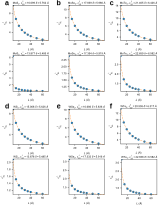
\includegraphics[width=0.95\linewidth]{img/SI-rescale-PRB.pdf}
  \caption{ Calculated (blue dots) and fitted
    (orange broken lines) $\varepsilon_{\mathrm{SL}}$ as function of
    $L$ for the group 6 TMDCs:
    \textbf{a}. MoS$_{2}$. \textbf{b}. MoSe$_{2}$. \textbf{c}.
    MoTe$_{2}$. \textbf{d}. WS$_{2}$. \textbf{e}. WSe$_{2}$. \textbf{f}.
    WTe$_{2}$. The extracted values of $\varepsilon_{\mathrm{2D}}$ and
    $\delta_{\mathrm{2D}}$ are shown in each subfigure.}
  \label{fig:rescale-prb}
\end{figure}

As can be seen from the fitted results in Figure
\ref{fig:rescale-prb}, the values of $\delta_{\mathrm{2D}}$ extracted
from both $\varepsilon_{\mathrm{SL}}^{\parallel}$ and
$\varepsilon_{\mathrm{SL}}^{\perp}$ are close when $L> 15$
{\AA}. Notably, the $\delta_{\mathrm{2D}}$ values are generally 10\%
smaller than the interlayer distance in corresponding bulk materials
$L_{\mathrm{bulk}}$ , as shown in Table \ref{tab:delta-L-DFt}. On the
other hand, the extracted $\delta_{\mathrm{2D}}$ values are closer to
the covalent thickness $\delta_{\mathrm{2D}}^{\mathrm{cov}}$ as
described in the main text, with a difference generally smaller than
5\%. Our results indicate that the conventional estimation of the 2D
layer thickness by its bulk interlayer distance
\cite{Matthes_2016,Laturia_2018}, will always lead to
overestimation. On the contrary, the out-of-plane polarizability
$\alpha_{\mathrm{2D}}^{\perp}$ correctly captures the thickness nature
of 2D materials.

\begin{table}[htbp]
  \centering
  \begin{tabular}[htbp]{lccccc}
  \hline{}
  Material & $\delta_{\mathrm{2D}}$ from $\varepsilon_{\mathrm{SL}}^{\parallel}$ ({\AA}) & $\delta_{\mathrm{2D}}$ from $\varepsilon_{\mathrm{SL}}^{\perp}$ ({\AA})& $L_{\mathrm{bulk}}$ ({\AA}) & $\delta_{\mathrm{2D}}^{\mathrm{cov}}$ ({\AA}) & $\alpha^{\perp}/\varepsilon_{0}$ ({\AA})\\
  \hline{}
  2H-MoS$_{2}$ & 5.76 & 5.49 & 6.15 & 5.22 & 4.98\\
  2H-MoSe$_{2}$ & 5.98 & 5.92 & 6.46 &  5.73 & 5.60\\
  2H-MoTe$_{2}$ & 6.43 & 6.85 & 6.98 & 6.37 & 6.12\\
  2H-WS$_{2}$ & 5.63 & 5.49 & 6.15 & 5.20 & 5.00\\
  2H-WSe$_{2}$ & 5.84 & 5.92 & 6.49 & 5.75 & 5.42\\
  2H-WTe$_{2}$ & 6.32 & 6.58 & 7.06 & 6.38 & 6.33\\
  \hline{}
\end{tabular}

\caption{Calculated $\delta_{\mathrm{2D}}$ from
  $\varepsilon_{\mathrm{SL}}^{\parallel}$ and
  $\varepsilon_{\mathrm{SL}}^{\perp}$, compared with the interlayer
  distance of corresponding bulk material $L_{\mathrm{SL}}$, the
  covalent thickness $\delta_{\mathrm{2D}}^{\mathrm{cov}}$, and
  $\alpha^{\perp}/\varepsilon_{0}$ for 2H TMDC materials.}
\label{tab:delta-L-DFt}
\end{table}

Another drawback of the 2D dielectric constant approach is the
overestimation of the out-of-plane dielectric response. As can be seen
in Figure \ref{fig:rescale-prb}, the extracted
$\varepsilon_{\mathrm{2D}}^{\perp}$ values for the TMDCs studied
are comparable or even larger than
$\varepsilon_{\mathrm{2D}}^{\parallel}$, which does not agree with the
physical picture that electrostatic screening of 2D materials are much
smaller perpendicular to the 2D plane. In fact, combining
Eq. \ref{eq:MG-effect-1} and the definition of $\alpha^{\perp}$, we
have:
\begin{equation}
  \label{eq:eps-alpha-perp}
  \frac{\alpha^{\perp}}{\varepsilon_{0}} = \delta_{\mathrm{2D}}(1 - (\varepsilon_{\mathrm{2D}}^{\perp})^{-1})
\end{equation}

\begin{figure}[htbp]
  \centering
  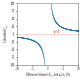
\includegraphics[width=0.7\linewidth]{img/SI-eps-alpha-error.pdf}
  \caption{Calculated $\varepsilon_{\mathrm{2D}}^{\perp}$ value as a
    function of the difference between $\delta_{\mathrm{2D}}$ and
    $\alpha^{\perp}/\varepsilon_{0}$. A small change of
    $\alpha^{\perp}/\varepsilon_{0}$ chosen may lead to divergence of
    the $\varepsilon_{\mathrm{2D}}^{\perp}$ or even negative values,
    which is apparently unphysical}
  \label{fig:eps-alpha-error}
\end{figure}

which indicate that the characteristic length
$\alpha^{\perp}/\varepsilon_{0}$, is very close but slightly smaller
than $\delta_{\mathrm{2D}}$ estimated by the effective medium theory,
if $\varepsilon^{\perp}_{\mathrm{2D}} \gg 1$. Moreover, from
Eq. \ref{eq:eps-alpha-perp}, when $\delta_{\mathrm{2D}}$ and
$\alpha^{\perp}/\varepsilon_{0}$ are close, slight change of the
$\delta_{\mathrm{2D}}$ chosen may lead to divergence of
$\varepsilon_{\mathrm{2D}}^{\perp}$, as shown in Figure
\ref{fig:eps-alpha-error}. Therefore cautions must to taken when
treating the dielectric response of the 2D material using effective
medium theory. In comparison, the 2D polarizability does not require
the guess of the thickness, and therefore is the true descriptor of
the 2D dielectric nature.

To conclude, based on theoretical and technical considerations, there are several
advantages of using the polarizability $\alpha$ for describing the dielectric
nature of 2D materials, including
\begin{enumerate}
\item $\alpha$ can be used to describe both the local and macroscopic dielectric properties, while $\epsilon_{\mathrm{2D}}$ can't.
\item Calculating $\alpha$ only requires to calculate the dielectric response at single superlattice length, while $\epsilon_{\mathrm{2D}}$ requires calculation with varied superlattice length.
\item $\alpha$ correctly respresents the screening length of 2D material, while $\epsilon_{\mathrm{2D}}$ does not.
\item $\alpha$ correctly represents the different degree of screening in/out-of-plane, while $\epsilon_{\mathrm{2D}}$ does not.
  
\item The value of $\epsilon_{\mathrm{2D}}$ hugely depends on the
  choice of the thickness of 2D material, while such information is
  intrinsically embedded in $\alpha$.
\end{enumerate}





\section{Further analysis of the 2D polarizability}
\label{sec:pol-2D}

In this section we will provide more analysis on the 2D polarizability
in addition to the main text.

\subsection{Dependence of superlattice size}
\label{sec:pol-2D-1}

We study the polarizabilties of group 6 TMDCs to demonstrate the
dependency between the 2D polarizability $\alpha$ and the superlattice
length $L$, which is shown in Figure \ref{fig:eps-L-all} \todo{Which
  method?}.  In all cases, we observe that the calculated
polarizability converges when $L>$15 \AA{}, in good agreement with our
conclusion in main text. The lower bound of $L_{\mathrm{min}}$ for the
convergence of $\alpha$ can be viewed as the minimal distance that
overlap of induced charge density from image layers is negligible. In
practice, any superlattice size larger than $L_{\mathrm{min}}$ can be
used for calculating the intrinsic 2D dielectric nature through the
polarizability, however to reduce the computational cost, especially
at the HSE level, we typically choose a superlattice size no larger
than 35 \AA{}.

\begin{figure}[htbp]
  \centering
  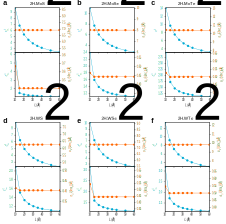
\includegraphics[width=0.95\linewidth]{img/SI-eps-L-all.pdf} 
  \caption{Calculated value of $\varepsilon_{\mathrm{SL}}^{\parallel}$
    (top left axis), $\varepsilon_{\mathrm{SL}}^{\perp}$ (bottom left
    axis), $\alpha^{\parallel}$ (top right axis) and $\alpha^{\perp}$
    (bottom right axis) of various group 6 TMDCs. In all cases, the
    polarizability  converges when $L>$15 \AA{}}
  \label{fig:eps-L-all}
\end{figure}


\subsection{Depdence of bandgap}
\label{sec:pol-2D-2}

In this section we further look into the bandgap dependency of the 2D
polarizability. Figure \ref{fig:SI-raw-HSE} shows $\alpha^{\parallel}$
and $\alpha^{\perp}$ as functions of $E_{\mathrm{g}}$ of the 2D
materials studied here. We observe that $\alpha^{\parallel}$ can be
approximated by a reciprocal function of $E_{\mathrm{g}}$, that
$\alpha^{\parallel}\sim{} 7.295(E_{\mathrm{g}})^{-1}$. On the other
hand, the plot of $\alpha^{\perp}$ against $E_{\mathrm{g}}$ shows no
apparent correlation.
\begin{figure}[htbp]
  \centering
  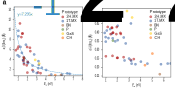
\includegraphics[width=0.8\linewidth]{img/SI-alpha_EG_raw_HSE.pdf}
  \caption{$E_{\mathrm{g}}$-dependence of    \textbf{a} $\alpha^{\parallel}$ and
    \textbf{b} $\alpha^{\perp}$ for the 2D materials investigated here.}
  \label{fig:SI-raw-HSE}
\end{figure}

\begin{figure}[htbp]
  \centering
  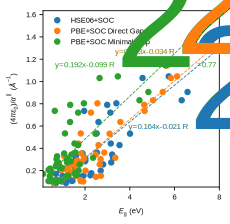
\includegraphics[width=0.5\linewidth]{img/SI-compare_alpha_Eg.pdf}
  \caption{Relation between $1/\alpha^{\parallel}$ and various choices
    of $E_{\mathrm{g}}$: minimal gap from HSE06 (blue), minimal gap
    from PBE (orange) and direct gap from PBE (green). The linear
    regression results are shown as broken lines.}
  \label{fig:alpha-Eg-diff}
\end{figure}

We also investigate the relation of 2D polarizabilities with
difference choices of \textit{ab initio} bandgaps. It is widely
accepted that the PBE method, while gives quantitative predictions of
the dielectric response of 2D and layered materials, tends to
underestimate the bangap
\cite{Kumar_2016_PRB,Kumar_2016_jpcc}. \todo{complete the discussion
  for HSE?}  Indeed, changing the choice of $E_{\mathrm{g}}$ yields
different regression relation with $1/\alpha^{\parallel}$, as shown in
Figure \ref{fig:alpha-Eg-diff}. We see that due to the underestimation
of PBE bandgap, the slope of linear regression is larger than that
from HSE-bandgap. We also observe that the $1/\alpha-E_{\mathrm{g}}$
relation is better presented by using the minimal HSE bandga than the
minimal PBE bandgap, due to higher regression $R^{2}$ coefficient of
the former. We note that the higher $R^{2}$ coefficient observed using
the direct PBE bandgap than the minimal PBE bandgap may be solely
caused by the fact that the direct bandgap of 2D materials on the PBE
level is closer to the HSE bandgap. From the random phase
approximation theory of dielectric response, the polarizability is
contributed by all possible transition between valence and conduction
bands, with the minimal bandgap as the least possible transition. In
this sense, $\alpha^{\parallel}$ is mostly like to be associated with
the minimal, not direct bandgap, as also observed in the original Moss
relation. We also examine the validity of such statement based on the
analysis of the Computational 2D Materials Database (C2DB)
\cite{Haastrup_2018}, as will be discussed in the following sections.








\section{Validation on the C2DB 2D materials database}
\label{sec:gpaw}
\subsection{Validation of the universal description of 2D polarizabilities}
\label{sec:gpaw-1}

\begin{figure}[htbp]
  \centering
  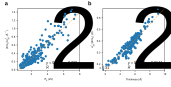
\includegraphics[width=0.8\linewidth]{img/SI-gpaw-data.pdf}
  \caption{Validation the linear relation between \textbf{a}
    $1/\alpha^{\parallel}-E_{\mathrm{g}}(\mathrm{HSE})$ and \textbf{b}
    $\alpha^{\perp}-\delta_{\mathrm{2D}}^{\mathrm{cov}}$ on the C2DB
    2D material database. }
  \label{fig:gpaw-alpha-relation}
\end{figure}

Due to the high computation complexity of dielectric response
calculations on the HSE level, our 2D material database is limited to
about 50 types of materials. It is desirable to validate our proposed
relations on a even larger scale database. \todo{Add comments for the
  C2DB database}. We select 210 semiconducting 2D materials from the
C2DB database with a HSE bandgap larger than 0.5 eV and extracted the
2D polarizabilities calculated on the PBE level. The propsed linear
relations between $1/\alpha^{\parallel}-E_{\mathrm{g}}(\mathrm{HSE})$
and $\alpha^{\perp}-\delta_{\mathrm{2D}}^{\mathrm{cov}}$ are also
valid, as shown in Figure \ref{fig:gpaw-alpha-relation}. Excellent
linear correlation is observed in both cases, with the $R^{2}$
coefficient larger than 0.9, indicating the existence of the universal
description of 2D dielectric nature through the proposed relations
with the 2D polarizabilities. We note that the slope of linear
regression is slightly different from the our proposed relation from
the dielectric response on HSE level, due to the fact that the
macroscopic dielectric constant $\varepsilon_{\mathrm{SL}}$ calculated
on the PBE level is about 5\% lower. Despite the minor deviation of
the slope of linear regression, the analysis on the C2DB database
supports our understanding of the universal dielectric nature of 2D
materials.

\subsection{Choice of bandgap}
\label{sec:gpaw-2}

Next we investigate the influence of choice of $E_{\mathrm{g}}$ on the
regression of $\alpha^{\parallel}-E_{\mathrm{g}}$ relation. Figure
\ref{fig:SI-gpaw-alpha-Eg-all} shows $1/\alpha^{\parallel}$ from the
C2DB database as a function of minimal and direct bandgap calculated
on PBE, HSE and GW levels.\todo{to be more specific?} We observe,
although the regression $R^{2}$ coefficient in all cases are around
0.9, the $\alpha^{\parallel}-E_{\mathrm{g}}$ is better described using
the HSE and GW bandgaps than the PBE bandgaps. On the other hand,
using indirect or minimal bandgaps on the same level gives almost
identical regression slope. The observations are in good agreement
with our calculations on the HSE level discussed in Section
\ref{sec:pol-2D-2}. In combination with the physical contribution of
$E_{\mathrm{g}}$ to the dielectric screening, we conclude that the
minimal bandgap should be used for quantitative prediction of the
in-plane 2D polarizability. The prediction is greatly improved when
more accurate theory level for bandgap is used (for instance, HSE and GW).

\begin{figure}[htbp]
  \centering
  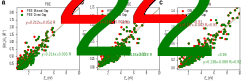
\includegraphics[width=0.95\linewidth]{img/SI-gpaw-alpha_Eg_all.pdf}
  \caption{$\alpha^{\parallel}$ as funtion of minimal and direct
    $E_{\mathrm{g}}$ calculated on different theoretical levels:
    \textbf{a} PBE, \textbf{b} HSE and \textbf{c} GW of the C2DB
    database.}
  \label{fig:SI-gpaw-alpha-Eg-all}
\end{figure}

\subsection{Relation between 2D polarizabilities and other physical quantities}
\label{sec:gpaw-3}

The relatively large size of the C2DB 2D materials database allows us
to examine the relation between 2D polarizabilities and other physical
quantities. We choose the following quantities for comparison,
corresponding to Figures \ref{fig:gpaw-2D-quantities-1} to
\ref{fig:gpaw-2D-quantities-3}:
\begin{enumerate}
\item The effective carrier mass for electron $m_{e}^{*}$ and hole $m_{h}^{*}$
  
\item The quantum capacitance at the conduction band edge
  $C_{\mathrm{Q}}^{\mathrm{C}}$ and valence band edge
  ($C_{\mathrm{Q}}^{\mathrm{V}}$).

  
\item The total atomic polarizabilities per area $\alpha^{\mathrm{sum}}$.
\end{enumerate}
\begin{figure}[htbp]
  \centering
  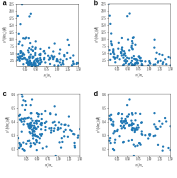
\includegraphics[width=0.75\linewidth]{img/SI-gpaw-alpha-emass.pdf}
  \caption{Relation between 2D polarizabilities and the effective
    carrier mass from the C2DB 2D material
    database. \textbf{a}. $\alpha^{\parallel}$ as a function of the
    electron mass $m_{e}^{*}$.  \textbf{b}. $\alpha^{\parallel}$ as a
    function of the hole mass
    $m_{h}^{*}$. \textbf{c}. $\alpha^{\perp}$ as a function of the
    electron mass $m_{e}^{*}$.  \textbf{d}. $\alpha^{\perp}$ as a
    function of the hole mass $m_{h}^{*}$. No apparent correlation
    between the 2D polarizabilities and the effective carrier masses
    is observed.}
  \label{fig:gpaw-2D-quantities-1}
\end{figure}

\begin{figure}[htbp]
  \centering
  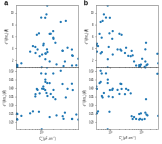
\includegraphics[width=0.6\linewidth]{img/SI-quantum-capacitance.pdf}
  \caption{Relation between the 2D polarizabilities with the quantum
    capacitance. \textbf{a} $\alpha^{\parallel}$ (top) and
    $\alpha^{\perp}$ (bottom) as functions of the quantum capacitance
    of the conduction band edge,
    $C_{\mathrm{Q}}^{\mathrm{C}}$. \textbf{b} $\alpha^{\parallel}$
    (top) and $\alpha^{\perp}$ (bottom) as functions of the quantum
    capacitance of the valence band edge,
    $C_{\mathrm{Q}}^{\mathrm{V}}$. Similar to the case of effective
    carrier mass, no apparent correlation between 2D polarizabilities
    and the quantum capacitance can be found.}
  \label{fig:gpaw-2D-quantities-2}
\end{figure}

\begin{figure}[htbp]
  \centering
  
\includegraphics[width=0.75\linewidth]{img/SI-gpaw-alpha-atomic-polarizability.pdf}
  \caption{Relation between the 2D polarizabilities
    (\textbf{a}. $\alpha^{\parallel}$ and
    \textbf{b}. $\alpha^{\perp}$) with the total atomic polarizability per area.}
  \label{fig:gpaw-2D-quantities-3}
\end{figure}

The quantum capacitance
$C_{\mathrm{Q}}(E)$ at certain energy level $E$ is calculated using
the relation $C_{\mathrm{Q}}(E)=\mathrm{DOS}(E)e^{2}$, where
$\mathrm{DOS}(E)$ is the density of states at the conduction or valence band edge (averaged by cell
area). The DOS value is calculated at the energy level with a charge
cutoff such that
$|n_{\mathrm{2D}}(E)| = 5 \times 10^{13}\ \mathrm{cm}^{-2}$, calculated by
the relation of accumulated charge $n_{\mathrm{2D}}(E)$ at CB or VB:
\begin{equation}
  \label{eq:CQ-method}
  |n_{\mathrm{2D}}(E)| = \left|\int_{E_{\mathrm{BE}}}^{E} \mathrm{DOS}(E') dE' \right|
\end{equation}
where $E_{\mathrm{BE}}$ is the energy of the CB or VB band edge.

The total polarizability $\alpha^{\mathrm{sum}}$ is calculated by the
summation of the atomic polarizabilities $\alpha^{\mathrm{atom}}$
\cite{Gould_2016_jctc} of individual atoms per area $A$, such that:
\begin{equation}
  \label{eq:atom-polar}
  \alpha^{\mathrm{sum}} = \frac{\sum_{i} \alpha^{\mathrm{atom}}_{i}}{A}
\end{equation}

From Figures \ref{fig:gpaw-2D-quantities-1} to
\ref{fig:gpaw-2D-quantities-3} we can see that none of the above
quantities have apparent relation with the 2D polarizabilities, as
compared with the bandgap and covalent thickness proposed in the main
text. \todo{add some more explanation}




\section{More theoretical analysis}
\label{eq:MG-effect-1}

\subsection{Detailed derivations from Eq. 10}
\label{sec:theory-1}

Here we will first show how Eq. 10 in the main text is
derived. Treating the in-plane wavefunctions as plane wave with form
$\psi^{\parallel}(\rho) \propto e^{i \mathbf{k \rho}}$, the matrix
element of
$<\psi_{\mathrm{v}}(\mathbf{k})|e^{-i\mathbf{qr}}|\psi_{\mathrm{c}}(\mathbf{k+q})>$,
when $\mathbf{q}=(0, 0, q_{z})$, becomes\cite{Hybertsen_1987}:
\begin{equation}
  \begin{aligned}
    \label{eq:matrix-z}
  <\psi_{\mathrm{v}}(\mathbf{k})|e^{-i\mathbf{qr}}|\psi_{\mathrm{c}}(\mathbf{k+q})>
  &= \frac{1}{A} \int dx \int dy
  e^{i(\mathbf{-k \rho} - \mathbf{q \rho} + \mathbf{(k+q) \rho})}
  \int (\psi^{\perp})^{*}_{\mathrm{v}}(\mathbf{k})e^{-iq_{z}z}\psi^{\perp}_{\mathrm{c}}(\mathbf{k+q})\\
  &= <\psi^{\perp}_{\mathrm{v}}(\mathbf{k})|e^{-iq_{z}z}|\psi^{\perp}_{\mathrm{c}}(\mathbf{k+q})>
  \end{aligned}
\end{equation}
Note that the states perpendicular are bound, the integral is
meaningful only when $\mathbf{k=k+q}$ \cite{davies_physics_1997}. By
performing the Taylor expansion of
$e^{-i\mathbf{qr}} \approx 1 - i\mathbf{qr}$, we get:
\begin{equation}
  \begin{aligned}
    \label{eq:matrix-z}
    <\psi^{\perp}_{\mathrm{v}}(\mathbf{k})|e^{-iq_{z}z}|\psi^{\perp}_{\mathrm{c}}(\mathbf{k})>
    &\approx <\psi^{\perp}_{\mathrm{v}}(\mathbf{k})|\psi^{\perp}_{\mathrm{c}}(\mathbf{k})> -
    iq_{z} <\psi^{\perp}_{\mathrm{v}}(\mathbf{k})|z|\psi^{\perp}_{\mathrm{c}}(\mathbf{k})>\\
    &= -iq_{z} <\psi^{\perp}_{\mathrm{v}}(\mathbf{k})|z|\psi^{\perp}_{\mathrm{c}}(\mathbf{k})>
   \end{aligned}
\end{equation}
plug this into Eq. 7 in main text and express the summation over
$k_{x}$ and $k_{y}$ in a continuous form within the Brillouin Zone, we
arrive at Eq. 10 in main text.

Although the exact form for $\psi^{\perp}$ depends on the exact
distribution of $V(z)$, without loss of generality we can assume the
electrons are confined in a potential well of width $\delta$, which is
the typical treatment for semiconductor QWs
\cite{ihn_semiconductor_2009}. The allowed bound states inside the
confined region generally has wave vector
$k_{z} \propto n \pi / \delta$. With the total energy
$E_{n}(\mathbf{k}) = {\displaystyle \frac{\hbar^{2} (k_{x}^{2} +
    k_{y}^{2})}{2 m^{\parallel}} + \frac{\hbar^{2} n^{2} \pi^{2}}{2
    m^{\perp} \delta^{2}}}$, where $m^{\parallel}$ and $m^{\perp}$ are
the effective masses parallel and perpendicular to the 2D
plane. Therefore the denominator of Eq. 10 becomes independent of
$\mathbf{k}$, that
$E_{\mathrm{c}}(\mathbf{k}) - E_{\mathrm{v}}(\mathbf{k}) =
(n_{\mathrm{c}}^{2} - n_{\mathrm{v}}^{2}) {\displaystyle
  \frac{\hbar^{2} \pi^{2}}{2 m^{\perp} \delta^{2}}}$. On the other
hand, the numerator
$<\psi^{\perp}_{\mathrm{v}}(\mathbf{k})|z|\psi^{\perp}_{\mathrm{c}}(\mathbf{k})>$
is proportional to the confinement length $\delta$ (can be seen using
particle-in-box solution\cite{davies_physics_1997}). In combination,
the individual terms of the summation in the right hand of Eq. 10 is
independent of neither $E_{\mathrm{g}}$ nor \textbf{k}, proving that
$\alpha^{\perp}$ is independent of the band gap.

Finally we will show the $\alpha^{\perp}$ is related to the
confinement length $\delta$, or equivalent the thickness of the 2D
material. For simplicity we assume $\psi^{\parallel}$ is the solution
of a particle confined inside an infinite potential well of width
$\delta$ with the form $\psi \propto \sin(\frac{n\pi}{\delta})$. At 0
K, the only non-zero contribution for the transition between band
$n_{\mathrm{v}}$ and $n_{\mathrm{c}}$ corresponds with in-plane wave
vector $\mathbf{k}_{\rho}$ within the range of $k_{\mathrm{F}}^{\mathrm{v}}$ to
$k_{\mathrm{F}}^{\mathrm{c}}$, the Fermi vectors of each band. Therefore we have:
\begin{equation}
  \begin{aligned}
    \alpha^{\perp} &\propto \delta^{4} m^{\perp} \int
    d^{2}\mathbf{k}_{\rho}
    \frac{f(\psi_{\mathrm{v}}(\mathbf{k}_{\rho}))
      -f(\psi_{\mathrm{v}}(\mathbf{k}_{\rho})) }{n_{\mathrm{c}}^{2} -
      n_{\mathrm{v}}^{2}}\\
    &= \delta^{4} m^{\perp} \sum_{\mathrm{c, v}}\pi \frac{
      (k_{\mathrm{F}}^{\mathrm{c}})^{2} -
        (k_{\mathrm{F}}^{\mathrm{v}})^{2}}{n_{\mathrm{c}}^{2} -
        n_{\mathrm{v}}^{2}}
  \end{aligned}
\end{equation}
Since the Fermi wave vector for band \textit{i} follows
${\displaystyle
  \frac{\hbar^{2}(k_{\mathrm{F}}^{i})^{2}}{2m^{\parallel}}} +
{\displaystyle \frac{\hbar^{2} n_{i}^{2} \pi^{2}}{2m^{\perp}
    \delta^{2}}} = E_{\mathrm{F}}$, we have
$ (k_{\mathrm{F}}^{\mathrm{c}})^{2} -
(k_{\mathrm{F}}^{\mathrm{v}})^{2} \propto (n_{\mathrm{c}}^{2} -
n_{\mathrm{v}}^{2}) {\displaystyle
  \frac{m^{\parallel}}{m^{\perp}}}$. Note that in the particle-in-box
model, the energy levels for a sub-nm QW will be at the order of 10
eV, which allows only few states inside the QW. Combine with the fact
that the strongest transition comes from the lowest bands
\cite{davies_physics_1997}, we can finally show:
\begin{equation}
  \label{eq:alpha-perp-L}
  \alpha^{\perp} \propto m^{\parallel} \delta^{2}
\end{equation}
Apart from the power of $\delta$, this explains our observation
$\alpha^{\perp}$ is related with the thickness of a 2D material. We
note the power law of $\delta^{2}$ instead of $\delta$ is
inevitable. The atomic polarizabilities of free particles inside a 1D
infinite QW, finite QW or harmonic QW all show dependency with
$\delta^{4}$, where $\delta$ is the length of confinement or effective
harmonic length of the QW \cite{Fowler_1984,Maize_2011}. Since the 2D
polarizability is the molecular polarizability divided by the area,
such approach will always yield $\alpha^{\perp} \propto \delta^{2}$
regardless of the Hamiltonian used. To accurately model the
$\alpha^{\perp}$ we need a better model for the confinement in
z-direction than simple square potential well, which may be
tedious. Nevertheless the simple model presented here still captures
the bandgap-indepent and thickness-related feature of
$\alpha^{\perp}$, supporting our findings in the main text.

\subsection{Detailed discussion for main text Eq. 14 }
\label{sec:theory-2}

Eq. 14 is the detailed form of Eq. 6 considering wavefunctions in all
directions are periodic which can be written in the form of Block
waves. The solution for Eq. 14 in main text is derived as follows. For
simplicity we consider that the effective mass $m^{*}$ is uniform,
which is generally a good assumption for bulk materials. Considering
only one pair of valence-conduction transition, and take the result
from \cite{Jiang_2017_Eg_Eb}, we get:
\begin{equation}
  \begin{aligned}
    \label{eq:eps-bulk}
    \varepsilon_{\mathrm{bulk}} - 1 &\propto \int d^{3}\mathbf{k}
    {\displaystyle \frac{1}{(E_{\mathrm{g}} + {\displaystyle
          \frac{\hbar^{2} k^{2}}{m^{*}}})^{2}}}\\
    &= \int_{0}^{k_{\mathrm{BZ}}} {\displaystyle
      \frac{4 \pi k^{2}}{(E_{\mathrm{g}} + {\displaystyle \frac{\hbar^{2}
            k^{2}}{m^{*}}})^{2}}} dk
  \end{aligned}
\end{equation}
where $k_{\mathrm{BZ}}$ is the boundary for the Brillouin Zone. The
last step in Eq. \ref{eq:eps-bulk} assumes the integral within the
Brillouin Zone is equivalent to integral inside a sphere of
k-space. Let $\hbar^{2}/(2 m^{*})=A$, the integral becomes:
\begin{equation}
  \begin{aligned}
    \label{eq:integral-BZ-bulk}
    \alpha^{\perp} &\propto {\displaystyle \frac{2 \pi
        \mathrm{arctan}(\sqrt{Ak^{2}/E_{\mathrm{g}}})}{\sqrt{E_{\mathrm{g}}A^{3}}}
        - \frac{2\pi k}{A(A+E_{\mathrm{g}}k^{2})}
      } \bigg\rvert_{0}^{k_{\mathrm{BZ}}}\\
      &\propto \sqrt{\frac{m^{*}}{E_{\mathrm{g}}}}
  \end{aligned}
\end{equation}
since generally
$\hbar^{2}k_{\mathrm{BZ}}^{2}/(2m^{*}) \gg E_{\mathrm{g}}$. When
$\varepsilon_{\mathrm{bulk}} \gg 1$ and assuming the difference
between $m^{*}$ in different semiconductors is small
\cite{Finkenrath_1988}, it is the Moss relation of bulk semiconductors.

\subsection{Static 2D polarizability and 2D plasma frequency}
\label{sec:omega-p}

A common approach for describing the bulk dielectric function of bulk
semiconductors is via the Lorentz oscillator model, where the
dielectric function is dominated by the plasma frequencies
$\omega_{\mathrm{3D}}^{\mathrm{p}}$ and bandgap $E_{\mathrm{g}}$ of
individual oscillators \cite{ketterson_physics_2016}. At zero optical
frequency and the static limit, the dielectric constant for single
oscillator is:
\begin{equation}
  \label{eq:eps-plas-3D}
  \varepsilon_{\mathrm{3D}} = 1 +
  \frac{\hbar^{2} (\omega_{\mathrm{3D}}^{\mathrm{p}})^{2}}{E_{\mathrm{g}}^{2}}
\end{equation}
where
$\omega_{\mathrm{3D}}^{\mathrm{p}} = {\displaystyle \sqrt{\frac{e^{2}
      n_{\mathrm{3D}}}{\varepsilon_{0} m_{e}}}}$, where
$n_{\mathrm{3D}}$ is the 3D number density of valence
electrons. Combine Eq. \ref{eq:eps-plas-3D} with Eq. 3 in main text,
we get:
\begin{equation}
  \begin{aligned}
  \label{eq:alpha-plas}
  \alpha^{\parallel} &= \frac{e^{2} n_{\mathrm{3D}} L}{m_{e} E_{\mathrm{g}}^{2}} \\
  &= \frac{e^{2} n_{\mathrm{2D}}}{m_{e} E_{\mathrm{g}}^{2}} \\
  &= \varepsilon_{0} \frac{\hbar^{2}
    (\omega_{\mathrm{2D}}^{\mathrm{p}})^{2}}{E_{\mathrm{g}}^{2}}
\end{aligned}
\end{equation}
where $n_{\mathrm{2D}} =n_{\mathrm{3D}} L$ is the 2D number density of
valence electrons and
$\omega_{\mathrm{2D}}^{p}=\omega_{\mathrm{3D}}^{p}\sqrt{L}$ is the 2D
plasma frequency at static limit \cite{Nazarov_2015_2D_3D}, as
discussed in the main text. Apparently $n_{\mathrm{2D}}$ and
$\omega_{\mathrm{2D}}^{p}$ defines the superlattice-independent 2D
quantity $\alpha^{\parallel}$, while its 3D counterpart
$\varepsilon_{\mathrm{3D}}$ is dependent on $L$. By defining the 2D
valence charge density
$\sigma_{\mathrm{2D}}^{\mathrm{v}}=n_{\mathrm{2D}}e$, we have also
calculated $\alpha^{\parallel}$ as a function of
$\sigma_{\mathrm{2D}}^{\mathrm{v}}/E_{\mathrm{g}}^{2}$ using the C2DB database, as shown in Figure \ref{fig:plasma}.
\begin{figure}[htbp]
  \centering
  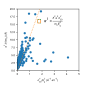
\includegraphics[width=0.65\linewidth]{img/SI-lorentz-model.pdf}
  \caption{Calculated$\alpha^{\parallel}$ as a function of
    $\sigma_{\mathrm{2D}}^{\mathrm{v}}/E_{\mathrm{g}}^{2}$ using the
    C2DB database. The broken line shows the theoretical prediction
    from single-oscillator model.}
  \label{fig:plasma}
\end{figure}
It can be seen that, a large number of materials are close to the
theoretical value of
$\alpha^{\parallel} = \frac{e^{2} n_{\mathrm{3D}} L}{m_{e}
  E_{\mathrm{g}}^{2}}$ (broken line). However there are also many
violations to this simple relation, making such model not suitable for
quantitative prediction of the 2D dielectric nature, due to the
oversimplification of single Lorentz oscillator. Nevertheless, this
example shows excellently how the quantities in both dimensions are
related to each other.

\section{Raw data from first principles calculations}
\label{sec:raw}

TBD.








\section*{}
\label{sec:ref}
\bibliography{ref}

\end{document}

